\chapter{Redes complejas}
\section{Grafos completos}
\subsubsection{\large Dibuja $L_i$, $i=1,...,8$} 
A continuación se muestran todos los grafos generados a partir del script del anexo.
\begin{figure}
	\centering
	\includegraphics[width=8cm]{grafo_completo_grado_1}
	\caption{Grafo $L_1$}
\end{figure}
\begin{figure}
	\centering
	\includegraphics[width=8cm]{grafo_completo_grado_2}
	\caption{Grafo $L_2$}
\end{figure}
\begin{figure}
	\centering
	\includegraphics[width=8cm]{grafo_completo_grado_3}
	\caption{Grafo $L_3$}
\end{figure}
\begin{figure}
	\centering
	\includegraphics[width=8cm]{grafo_completo_grado_4}
	\caption{Grafo $L_4$}
\end{figure}
\begin{figure}
	\centering
	\includegraphics[width=8cm]{grafo_completo_grado_5}
	\caption{Grafo $L_5$}
\end{figure}
\begin{figure}
	\centering
	\includegraphics[width=8cm]{grafo_completo_grado_6}
	\caption{Grafo $L_6$}
\end{figure}
\begin{figure}
	\centering
	\includegraphics[width=8cm]{grafo_completo_grado_7}
	\caption{Grafo $L_7$}
\end{figure}
\begin{figure}
	\centering
	\includegraphics[width=8cm]{grafo_completo_grado_8}
	\caption{Grafo $L_8$}
\end{figure}

\section{Multigrafo}
\subsubsection{\large Calcular la lista de aristas y la matriz de adyacencia para el multigrafo representado en la figura 5}
	Lista de aristas \begin{center}
		\begin{tabular}{ |c|c|c| } 
			\hline
			($n_1,n_2$) \\ 
			($n_2,n_1$) \\ 
			($n_2,n_3$)\\
			($n_2,n_4$)\\
			($n_4,n_4$)\\
			($n_4,n_3$)\\
			($n_3,n_5$)\\
			($n_5,n_4$)\\
			\hline
		\end{tabular}
	\end{center}
Matriz de Adyacencia:
$$\begin{pmatrix}
	0 & 1 & 0 & 0 & 0 \\ 
	1 & 0 & 0 & 0 & 0 \\ 
	0 & 1 & 0 & 1 & 0 \\ 
	0 & 1 & 0 & 1 & 1 \\ 
	0 & 0 & 1 & 0 & 0
\end{pmatrix}$$ 


\section{Grafo pesado}
\subsubsection{\large Calcular la lista de aristas y la matriz de adyacencia del grafo pesado que aparece en la figura 5}

Lista de aristas \begin{center}
	\begin{tabular}{ |c|c|c| } 
		\hline
		($n_1,n_2,5$) \\ 
		($n_2,n_3,1$)\\
		($n_2,n_4,6$)\\
		($n_3,n_5,5$)\\
		($n_4,n_3,3$)\\
		($n_5,n_4,1$)\\
		\hline
	\end{tabular}
\end{center}
Matriz de Adyacencia:
$$\begin{pmatrix}
0 & 0 & 0 & 0 & 0 \\ 
5 & 0 & 0 & 0 & 0 \\ 
0 & 1 & 0 & 0 & 0 \\ 
0 & 6 & 0 & 3 & 1 \\ 
0 & 0 & 5 & 0 & 0
\end{pmatrix}$$ 



\section{Grafo bipartito}
\subsubsection{\large Calcular la matriz de incidencia del grafo bipartito mostrado en el figura 6. Cual sería la matriz de incidencia si no existiera en dicho grafo el nodo m5 ?}


Matriz de Incidencia:
$$\begin{pmatrix}
0 & 1 & 1 & 0 & 0 \\ 
1 & 0 & 0 & 0 & 1 \\ 
0 & 0 & 0 & 0 & 1 \\ 
1 & 0 & 0 & 1 & 0 \\ 
0 & 1 & 0 & 0 & 0
\end{pmatrix}$$ 

Matriz de Incidencia sin nodo $m_5$:
$$\begin{pmatrix}
0 & 1 & 1 & 0  \\ 
1 & 0 & 0 & 0  \\ 
0 & 0 & 0 & 0  \\ 
1 & 0 & 0 & 1  \\ 
0 & 1 & 0 & 0 
\end{pmatrix}$$ 



\section{Grafo proyección 1}
\subsubsection{\large Dibujar el grafo proyección de nodos del grafo bipartito de la figura 6 y demostrar que el grafo proyección de nodos viene descrito por una matriz de adyacencia $P$ tal que $P = BB^T$}

\begin {center}
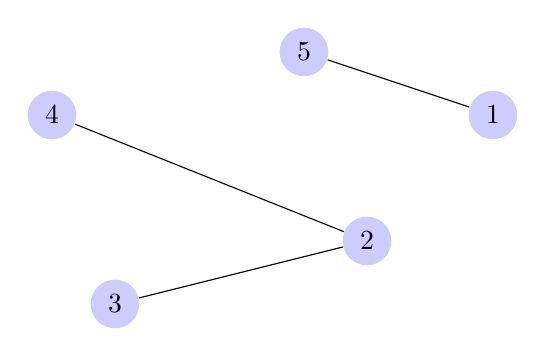
\begin{tikzpicture}
[scale=.8,auto=left,every node/.style={circle,fill=blue!20}]
\node (n4) at (4,8)  {4};
\node (n5) at (8,9)  {5};
\node (n1) at (11,8) {1};
\node (n2) at (9,6)  {2};
\node (n3) at (5,5)  {3};

\foreach \from/\to in {n1/n5,n2/n4,n2/n3}
\draw (\from) -- (\to);

\end{tikzpicture}
\end{center}

$$P=\begin{pmatrix}
	0 & 1 & 1 & 0 & 0 \\ 
	1 & 0 & 0 & 0 & 1 \\ 
	0 & 0 & 0 & 0 & 1 \\ 
	1 & 0 & 0 & 1 & 0 \\ 
	0 & 1 & 0 & 0 & 0
\end{pmatrix} . \begin{pmatrix}
0 & 1 & 0 & 1 & 0 \\ 
1 & 0 & 0 & 0 & 1 \\ 
1 & 0 & 0 & 0 & 0 \\ 
0 & 0 & 0 & 1 & 0 \\ 
0 & 1 & 1 & 0 & 0
\end{pmatrix}= \begin{pmatrix}
0 & 0 & 0 & 0 & 1 \\ 
0 & 0 & 1 & 1 & 0 \\ 
0 & 1 & 0 & 0 & 0 \\ 
0 & 1 & 0 & 0 & 0 \\ 
1 & 0 & 0 & 0 & 0
\end{pmatrix} $$ 



\subsubsection{\large Dibujar el grafo proyección de grupos del grafo bipartito de la figura 6 y demostrar que el grafo proyección de grupos viene descrito por una matriz de adyacencia $P$ tal que $P = BB^T$}

\begin {center}
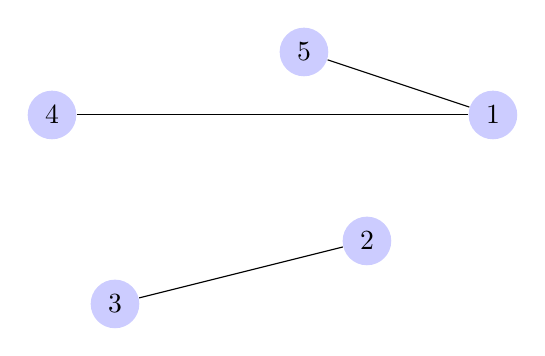
\begin{tikzpicture}
[scale=.8,auto=left,every node/.style={circle,fill=blue!20}]
\node (n4) at (4,8)  {4};
\node (n5) at (8,9)  {5};
\node (n1) at (11,8) {1};
\node (n2) at (9,6)  {2};
\node (n3) at (5,5)  {3};

\foreach \from/\to in {n1/n5,n1/n4,n2/n3}
\draw (\from) -- (\to);

\end{tikzpicture}
\end{center}


$$P=\begin{pmatrix}
0 & 1 & 0 & 1 & 0 \\ 
1 & 0 & 0 & 0 & 1 \\ 
1 & 0 & 0 & 0 & 0 \\ 
0 & 0 & 0 & 1 & 0 \\ 
0 & 1 & 1 & 0 & 0
\end{pmatrix}.\begin{pmatrix}
0 & 1 & 1 & 0 & 0 \\ 
1 & 0 & 0 & 0 & 1 \\ 
0 & 0 & 0 & 0 & 1 \\ 
1 & 0 & 0 & 1 & 0 \\ 
0 & 1 & 0 & 0 & 0
\end{pmatrix}= 
\begin{pmatrix}
0 & 0 & 0 & 1 & 1 \\ 
0 & 0 & 1 & 0 & 0 \\ 
0 & 1 & 0 & 0 & 0 \\ 
1 & 0 & 0 & 0 & 0 \\ 
1 & 0 & 0 & 0 & 0
\end{pmatrix} $$ 

\subsubsection{\large En un grafo simple no dirigido $k_i \in [0, N - 1]$, y en un red dirigida $k_i^{in}\in[0, N - 1]$ y $k_i^{out} \in [0, N - 1]$.}
\textit{Ejercicio propuesto en clase}

El resultado es evidente, puesto que en un grafo no dirigido como maximo el nodo puede estar conectado con todos los otros nodos, menos él mismo, lo cual hace que esté en un rango entre 0 ( si no esta conectado a nadie) y N-1 cuando esta conectado a todos los otros nodos.
En los otros casos, el razonamiento es el mismo puesto que se habla de grafos dirigidos y no multigrafos (en los cuales se llegaría hasta N)

\subsubsection{\large Se tiene que para una red simple $L=\frac{1}{2}\langle k\rangle N$}
\textit{Ejercicio propuesto en clase}

Tenemos por definición que: 
$$L=\frac{1}{2}\langle k\rangle N=\frac{1}{2}\frac{1}{N}(\sum_{i=1}^{N}\sum_{j=1}^{N}A_{ij}) N=\frac{1}{2}(\sum_{i=1}^{N}\sum_{j=1}^{N}A_{ij}) $$

donde la ultima igualdad es trivial puesto que en la matriz de adyacencia aparece el numero de aristas repetido dos veces.


\subsubsection{\large Calcular la distribución de probabilidad de grados del grafo no dirigido de la figura 5 y ver que está normalizada}
\begin{itemize}
\item $P(1)=1/5$
\item$P(2)=1/5$
\item $P(3)=3/5$
\end{itemize}
$P(1)+P(2)+P(3)=1$


\subsubsection{\large Calcular la distribución de probabilidad de grados del grafo dirigido y del multigrafo de la figura 5 y ver que está normalizada}
Grafo dirigido:

Saliente
\begin{itemize}
	\item $P(1)=4/5$
	\item$P(2)=1/5$

\end{itemize}
$P(1)+P(2)=1$

Entrante
\begin{itemize}
	\item $P(0)=1/5$
	\item$P(1)=2/5$
	\item $P(2)=2/5$

\end{itemize}
$P(1)+P(2)+P(0)=1$


Multigrafo:

Saliente
\begin{itemize}
	\item $P(1)=3/5$
	\item$P(2)=1/5$
	\item$P(3)=1/5$
\end{itemize}
$P(1)+P(2)+P(3)=1$

Entrante
\begin{itemize}
	\item $P(1)=3/5$
	\item$P(2)=1/5$
	\item $P(3)=1/5$
	
\end{itemize}
$P(1)+P(2)+P(3)=1$

\subsubsection{\large En el grafo no dirigido de la figura 5 calcular el número total de caminos cíclicos de longitud n = 3 que empiezan en los nodos }

$N=Traza\begin{pmatrix}
	0 & 1 & 0 & 0 & 0 \\ 
	1 & 0 & 1 & 1 & 0 \\ 
	0 & 1 & 0 & 1 & 1 \\ 
	0 & 1 & 1 & 0 & 1 \\ 
	0 & 0 & 1 & 1 & 0
	\end{pmatrix}^3=
	Traza\begin{pmatrix}
	0 & 3 & 1 & 1 & 2 \\ 
	3 & 2 & 6 & 6 & 2 \\ 
	1 & 6 & 4 & 5 & 5 \\ 
	1 & 6 & 5 & 4 & 5 \\ 
	2 & 2 & 5 & 5 & 2
	\end{pmatrix}=12$

Si el número nos parece grande, debemos recordar que no hablamos de caminos cíclicos auto evitados.

\subsubsection{\large Demostrar que para una red regular en forma de anillo donde cada nodo tiene grado k = 2m el coeficiente de agrupamiento es $C = 3(m - 1)/2(2m - 1)$}
Sea un grafo con grado $K=2m$

Para calcularlo el coeficiente de agrupamiento solo tenemos que tener en cuenta el numero de triángulos en el grafo de manera que uno de los nodos del triangulo sea nuestro nodo y el numero de tripletas en el grafo.

El numero de tripletas es el mismo que el de posibles links entre nodos vecinos de i, con lo que lo unico que tenemos que calcular es el orden del grafo completo que tuviese "m" links:
$$N_tripletas=\frac{2m(2m-1)}{2}=m(2m-1)$$

Para el numero de triángulos basta ver:

$$N_{triangulos}=3\sum_{j=0}^{m-1}j=3\frac{m(m-1)}{2}$$

Con lo cual, dividiendo por la formula que tenemos en los apuntes:
$$C=\frac{1}{N}\sum_{i=1}^{N}\frac{3(m - 1)}{2(2m - 1)}=\frac{3(m - 1)}{2(2m - 1)}$$
